\documentclass[t]{beamer}
%\documentclass[c]{beamer}
\listfiles

\definecolor{normalbg}{HTML}{EDF2FC}
\definecolor{normalfg}{HTML}{012528}
\definecolor{normalsymbol}{HTML}{012528}

\definecolor{examplebg}{HTML}{1098F7}%{A76571}%
\definecolor{alertbg}{HTML}{FAC05E}
\definecolor{myblue}{HTML}{DA4167}

\mode<presentation> {
    \usetheme[english,titlepage0,20pt]{KIT}
    \usefonttheme{structurebold}  
    %\useinnertheme[shadow=true]{rounded}
    %\setbeamercovered{transparent}
    \setbeamertemplate{navigation symbols}{}

    \setbeamertemplate{blocks}[rounded][shadow=true]
    \setbeamercolor{block title}{fg=normalfg, bg=normalbg}
    \setbeamercolor{block body}{fg=normalfg, bg=normalbg!20}
    \setbeamercolor{block title example}{fg=normalfg, bg=examplebg!50}
    \setbeamercolor{block body example}{fg=normalfg, bg=normalbg!20}
    \setbeamercolor{block title alerted}{fg=normalfg, bg=alertbg!50}
    \setbeamercolor{block body alerted}{fg=normalfg, bg=normalbg!20}

    \setbeamertemplate{itemize item}{\color{normalsymbol}\textbullet}
    \setbeamertemplate{itemize subitem}{\color{normalsymbol}\textbullet}
    \setbeamercolor{item projected}{bg=normalsymbol, fg=normalsymbol}

    \setbeamertemplate{itemize item}{\color{normalsymbol}\textbullet}
    \setbeamertemplate{itemize subitem}{\color{normalsymbol}\tiny\raise1.5pt\hbox{\donotcoloroutermaths$\blacktriangleright$}}
    \setbeamertemplate{itemize subsubitem}{\color{normalsymbol}\tiny\raise1.5pt\hbox{\donotcoloroutermaths$\blacktriangleright$}}
    \setbeamertemplate{enumerate item}{\color{normalsymbol}\small\insertenumlabel.}
    \setbeamertemplate{enumerate subitem}{\color{normalsymbol}\small\insertenumlabel.\insertsubenumlabel}
    \setbeamertemplate{enumerate subsubitem}{\color{normalsymbol}\small\insertenumlabel.\insertsubenumlabel.\insertsubsubenumlabel}
    \setbeamertemplate{enumerate mini template}{\color{normalsymbol}\small\insertenumlabel}
}


\usepackage[utf8]{inputenc}
\usepackage[TS1,T1]{fontenc}
\usepackage{babel}

\usepackage{array}
\usepackage{multicol}
\usepackage{multirow}
\usepackage{tabularx}
\usepackage{tabulary}

\usepackage{graphicx}
\usepackage{xcolor}
\usepackage{tikz}
\usetikzlibrary{positioning}
\usetikzlibrary{calc}
\usetikzlibrary{shapes}

\usepackage{background}

\usepackage{url}
\usepackage{hyperref}

\usepackage[ruled,linesnumbered,vlined]{algorithm2e}
\usepackage{amsmath}
\usepackage{amssymb}

\usepackage{mathtools}
\DeclarePairedDelimiter\ceil{\lceil}{\rceil}
\DeclarePairedDelimiter\floor{\lfloor}{\rfloor}
\DeclareMathOperator\hi{\ensuremath{\mathsf{hi}}}
\DeclareMathOperator\lo{\ensuremath{\mathsf{lo}}}

\DeclareMathOperator*{\argmax}{arg\,max}
\DeclareMathOperator*{\argmin}{arg\,min}

\newcommand{\verysmall}{\fontsize{6pt}{8.6pt}\selectfont}

\setlength{\leftmargini}{1em}
\setlength{\leftmarginii}{1em}


\title{Calculating Sufficient Reasons for Random Forest Classifiers}
\author{Markus Iser}
\subtitle{\insertauthor}
%\institute{Algorithm Engineering (Prof. Peter Sanders)\\Institute of Theoretical Informatics\\KIT Department of Informatics}
\institute{Algorithm~Engineering $\cdot$ Institute~of~Theoretical~Informatics}

\TitleImage[width=\titleimagewd]{scratch}

\begin{document}

\begin{frame}{asdf}
\maketitle
\end{frame}


\tikzset{
    invisible/.style={opacity=0},
    shady/.style={opacity=0.05},
    visible on/.style={alt={#1{}{shady}}},
    only on/.style={alt={#1{}{invisible}}},
    highlight on/.style={alt={#1{fill=alertbg!20,draw=alertbg,thick}{}}},
    high on/.style={alt={#1{fill=alertbg!20}{}}},
    alt/.code args={<#1>#2#3}{%
      \alt<#1>{\pgfkeysalso{#2}}{\pgfkeysalso{#3}} % \pgfkeysalso doesn't change the path
    },
}


\begin{frame}[fragile]{Reasoning about Learned Models}
\begin{tikzpicture}[remember picture, overlay, text=normalfg,
	blackbox/.style = {fill=black, text=white, minimum width=7em, minimum height=2em}, 
	whitebox/.style = {fill=white, text=normalfg, draw=alertbg, minimum width=7em, minimum height=2em}, 
	vertibox/.style = {rounded corners, text width=11em, text=examplebg, rotate=90}, 
	infobox/.style = {rounded corners, text=normalfg, fill=white, draw=alertbg, very thick, text depth=11em, text width=10em, font={\smaller}}]
	
%\fill [examplebg] (current page.north west) rectangle ($(current page.north east)!.2!(current page.south east)$) coordinate (a);

\fill [normalbg, rounded corners] ([yshift=2.7em, xshift=1em] current page.south west) rectangle ([yshift=-.3em,xshift=-1em] current page.east);
\node[vertibox] at ([xshift=2em,yshift=9em] current page.south west) () {Learning};

\node[blackbox] at ([yshift=-2em] current page.center) (model) {Model};
\node[whitebox, below=5em of model] (data) {Data};
\draw[->] (data) to[bend right] node[midway, right] {Train} (model);
\draw[->] (model) to[bend right] node[midway, left] {Evaluate} (data);

\node[whitebox, right=of model] (app) {Application};
\draw[->] (model) -- (app);

\fill [normalbg, rounded corners] ([yshift=-4em, xshift=1em] current page.north west) rectangle ([yshift=.5em,xshift=-1em] current page.east);
\node[vertibox] at ([xshift=2em,yshift=-6.5em] current page.north west) () {Reasoning};

\node[whitebox, above=of model] (symb) {Symbolic Representation};
\draw[->] (model) -- (symb);

\node[whitebox, above=of symb] (ana) {Static Analysis};
\draw[->] (ana) -- (symb);

\visible<2-> {
\node[above=1em of symb, xshift=-7em] {``What have you learned?''};
}
%\node[infobox, left=of ana, yshift=-4em] (ex) {Examples:
%\begin{itemize}
%\item asdf
%\end{itemize}
%};
%\draw[->] (ex) -- (ana);

\end{tikzpicture}
\end{frame}


\begin{frame}{Outline}

Prime Implicants of CNF Encoding of Random Forest Classifiers

\bigskip

\begin{block}{Contributions}

\begin{itemize}\setlength\itemsep{1em}
\item Monotonic CNF \emph{encoding} for random forest classifiers
\item \emph{Implementation} for \texttt{sklearn.ensemble.RandomForestClassifier}
\item \emph{Incremental method} to generate all prime implicants
\item First initial \emph{results}
\item Plenty of ideas for future work (paper is WIP)
\end{itemize}

\end{block}

\end{frame}


\begin{frame}{Decision Tree Classifiers}


\begin{tabular}{ccc}
	\bf Samples & \bf Classes & \bf Ground-truth\\[.5em]
	$T \subset \mathbb{R}^n$ & $K$ & $G \subset T \rightarrow K$\\
\end{tabular}

\begin{block}{Classification Problem}
Devise a prediction function $c : \mathbb{R}^n \rightarrow K$ maximizing the cardinality of correctly classified samples
\end{block}

\begin{alertblock}{Decision Tree Classifier}
A decision tree $\mathcal{D} = (V, E, f, t)$ is a \emph{binary tree} (V, E) with features $f : V \rightarrow \{1, 2, \dots, n\}$ and thresholds $t : V \rightarrow \mathbb{R}$
\end{alertblock}

\end{frame}


\begin{frame}{CNF Encoding Decision Tree Classifiers}

\begin{block}{Example \texttt{sklearn.tree.DecisionTreeClassifier}}

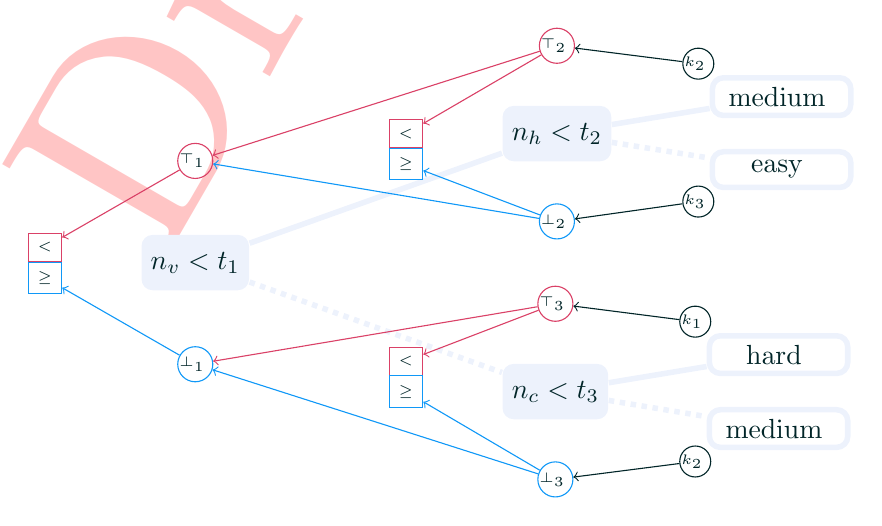
\begin{tikzpicture}[text=normalfg, 
	tree/.style = {fill=normalbg, rectangle, rounded corners, minimum width=2em, minimum height=2em}, 
    yes/.style = {draw=myblue, circle, align=center, inner sep=0em, minimum width=1em, text centered}, 
    no/.style = {draw=examplebg, circle, align=center, inner sep=0em, minimum width=1em, text centered}, 
    cl/.style = {draw=normalfg, circle, align=center, inner sep=0em, minimum width=1em, text centered}, 
    leaf/.style = {draw=normalbg, line width=2pt, rectangle, rounded corners, align=center, minimum width=5em, minimum height=1em},
    featl/.style = {draw=myblue, minimum width=1em, minimum height=1em},
    featr/.style = {draw=examplebg, minimum width=1em, minimum height=1em}]

% tree
\node[tree] (a1) { $n_v < t_1$ };
\node[tree, above right=3em of a1, xshift=7em, yshift=.5em] (b1) { $n_h < t_2$ };
\node[tree, below right=3em of a1, xshift=7em, yshift=-.5em] (b2) { $n_c < t_3$ };
\node[leaf, above right=5em of b1, yshift=-4em] (c1) { medium };
\node[leaf, below right=5em of b1, yshift=4em] (c2) { easy };
\node[leaf, above right=5em of b2, yshift=-4em] (c3) { hard };
\node[leaf, below right=5em of b2, yshift=4em] (c4) { medium };

\draw[draw=normalbg, line width=2pt] (a1) -- (b1);
\draw[draw=normalbg, line width=2pt] (b1) -- (c1);
\draw[draw=normalbg, line width=2pt] (b2) -- (c3);
\draw[draw=normalbg, line width=2pt, dotted] (a1) -- (b2);
\draw[draw=normalbg, line width=2pt, dotted] (b1) -- (c2);
\draw[draw=normalbg, line width=2pt, dotted] (b2) -- (c4);

\visible<2-> {
% bool nodes
\node[cl, above left=0em of c1] (k1) { \tiny $k_2$ };
\node[cl, above left=0em of c3] (k3) { \tiny $k_1$ };
\node[cl, below left=0em of c2] (k2) { \tiny $k_3$ };
\node[cl, below left=0em of c4] (k4) { \tiny $k_2$ };

\visible<3-> {
\node[yes, above=2em of a1] (a1true) { \tiny $\top_1$ };
\node[yes, above=1.5em of b1] (b1true) { \tiny $\top_2$ };
\node[yes, above=1.5em of b2] (b2true) { \tiny $\top_3$ };
\node[no, below=2em of a1] (a1false) { \tiny $\bot_1$ };
\node[no, below=1.5em of b1] (b1false) { \tiny $\bot_2$ };
\node[no, below=1.5em of b2] (b2false) { \tiny $\bot_3$ };
}

\visible<4-> {
\draw[<-, draw=examplebg] (a1false) -- (b2false);
\draw[<-, draw=normalfg] (b2false) -- (k4);
\draw[<-, draw=myblue] (a1false) -- (b2true);
\draw[<-, draw=normalfg] (b2true) -- (k3);
\draw[<-, draw=examplebg] (a1true) -- (b1false);
\draw[<-, draw=normalfg] (b1false) -- (k2);
\draw[<-, draw=myblue] (a1true) -- (b1true);
\draw[<-, draw=normalfg] (b1true) -- (k1);
}

\visible<5->{
% feature splits
\node[featl, left=of a1, yshift=.55em] (f1l) {\tiny $<$};
\node[featr, left=of a1, yshift=-.55em] (f1r) {\tiny $\geq$};
\draw[->, draw=myblue] (a1true) -- (f1l);
\draw[->, draw=examplebg] (a1false) -- (f1r);

\node[featl, left=of b1] (f2l) {\tiny $<$};
\node[featr, left=of b1, yshift=-1.1em] (f2r) {\tiny $\geq$};
\draw[->, draw=myblue] (b1true) -- (f2l);
\draw[->, draw=examplebg] (b1false) -- (f2r);

\node[featl, left=of b2, yshift=1.1em] (f3l) {\tiny $<$};
\node[featr, left=of b2] (f3r) {\tiny $\geq$};
\draw[->, draw=myblue] (b2true) -- (f3l);
\draw[->, draw=examplebg] (b2false) -- (f3r);
}
}
\end{tikzpicture}

\end{block}

\end{frame}


\begin{frame}{Encoding Feature Constraints}

\begin{block}{Multiple thresholds per feature}
\begin{itemize}
\item per feature collect thresholds and sort: $t_0 < t_1 < \dots < t_n$
\item one Boolean variable per interval (induced by thresholds)
\item $\mathcal{O}(n)$ encoding variables and clauses, only one clause per node
\item without encoding variables: quadratic growth
\end{itemize}
\end{block}

\begin{center}
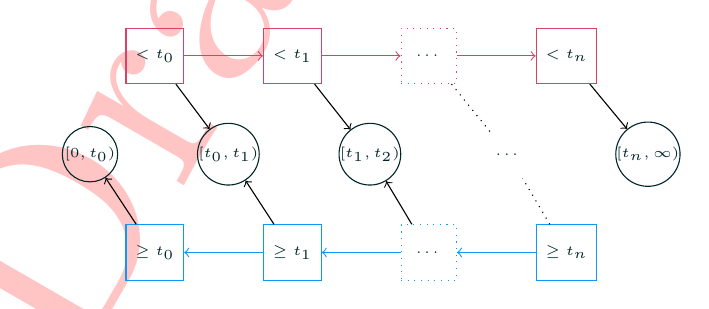
\begin{tikzpicture}[text=normalfg, 
	tree/.style = {fill=normalbg, rectangle, rounded corners, minimum width=2em, minimum height=2em}, 
    yes/.style = {draw=myblue, circle, align=center, inner sep=0em, minimum width=1em, text centered}, 
    no/.style = {draw=examplebg, circle, align=center, inner sep=0em, minimum width=1em, text centered}, 
    cl/.style = {draw=normalfg, circle, align=center, inner sep=0em, minimum width=1em, text centered}, 
    leaf/.style = {draw=normalbg, line width=2pt, rectangle, rounded corners, align=center, minimum width=5em, minimum height=1em},
    featl/.style = {draw=myblue, minimum width=2em, minimum height=2em},
    featr/.style = {draw=examplebg, minimum width=2em, minimum height=2em},
    inter/.style = {draw=normalfg, circle, align=center, inner sep=0em, minimum width=2em, minimum height=2em}]

\node (o) {};
\node[above=of o] (n) {};
\node[below=of o] (m) {};

\node[inter, right=of o, xshift=-2.3em] (f1i1) {\tiny $[0, t_0)$};
\node[inter, right=of f1i1] (f1i2) {\tiny $[t_0, t_1)$};
\node[inter, right=of f1i2] (f1i3) {\tiny $[t_1, t_2)$};
\node[inter, draw=none, right=of f1i3] (dots) {\tiny \dots};
\node[inter, right=of dots] (fli5) {\tiny $[t_n, \infty)$};

\visible<2->{
\node[featl, right=of n] (f1l1) {\tiny $<t_0$};
\node[featl, right=of f1l1] (f1l2) {\tiny $<t_1$};
\node[featl, dotted, right=of f1l2] (f1l3) {\tiny \dots};
\node[featl, right=of f1l3] (f1l4) {\tiny $<t_n$};
\draw[->, draw=myblue] (f1l1) -- (f1l2);
\draw[->, draw=myblue] (f1l2) -- (f1l3);
\draw[->, draw=myblue] (f1l3) -- (f1l4);

\node[featr, right=of m] (f1r1) {\tiny $\geq t_0$};
\node[featr, right=of f1r1] (f1r2) {\tiny $\geq t_1$};
\node[featr, dotted, right=of f1r2] (f1r3) {\tiny \dots};
\node[featr, right=of f1r3] (f1r4) {\tiny $\geq t_n$};
\draw[<-, draw=examplebg] (f1r1) -- (f1r2);
\draw[<-, draw=examplebg] (f1r2) -- (f1r3);
\draw[<-, draw=examplebg] (f1r3) -- (f1r4);

\draw[->] (f1r1) -- (f1i1);
\draw[->] (f1r2) -- (f1i2);
\draw[->] (f1r3) -- (f1i3);
\draw[dotted] (f1r4) -- (dots);

\draw[->] (f1l1) -- (f1i2);
\draw[->] (f1l2) -- (f1i3);
\draw[dotted] (f1l3) -- (dots);
\draw[->] (f1l4) -- (fli5);
}
\end{tikzpicture}
\end{center}
\end{frame}


\begin{frame}{Properties of the Encoding}

\begin{block}{Observations}

\begin{itemize}\setlength\itemsep{1em}
\item 2-SAT
\item Horn
\item Monotonic Circuit:\\[1em]
\begin{itemize}\setlength\itemsep{1em}
\item Classes are roots
\item Feature Intervals are leafs
\item Leafs are purely positive
\end{itemize}

\item Select a class by adding a unit-clause of the class variable, or select multiple classes by adding a disjunction of class variables
\end{itemize}

\end{block}

\end{frame}


\begin{frame}{Random Forest Classifiers}

\begin{tabular}{ccc}
	\bf Samples & \bf Classes & \bf Ground-truth\\[.5em]
	$T \subset \mathbb{R}^n$ & $K$ & $G \subset T \rightarrow K$\\
\end{tabular}

\begin{block}{Classification Problem}
Devise a prediction function $c : \mathbb{R}^n \rightarrow K$ maximizing the cardinality of correctly classified samples
\end{block}

\begin{alertblock}{Random Forest Classifier}
A \emph{random forest} $\mathcal{R}^d = \{ (T_i, \mathcal{D}_i) \mid 1 \leq i \leq d \}$ combines a set of $d$ decision trees. 
Each decision tree $\mathcal{D}_i$ is independently trained on randomly selected subsets of the training samples $T_i \subset T$
\end{alertblock}
\end{frame}


\begin{frame}{CNF Encoding Random Forest Classifiers}

\begin{block}{Example \texttt{sklearn.ensemble.RandomForestClassifier}}

\begin{itemize}\setlength\itemsep{1em}
\item each leaf $\ell$ has class probabilities $p_\ell(\mathsf{easy}), p_\ell(\mathsf{medium}), p_\ell(\mathsf{hard})$
\item each sample belongs to exactly one leaf in each of the trees
\item class is determined by $\argmax\limits_{k \in \{\mathsf{eas., med., h.}\}} \sum\limits_{\ell \in L} p_\ell(k)$
\end{itemize}

\bigskip

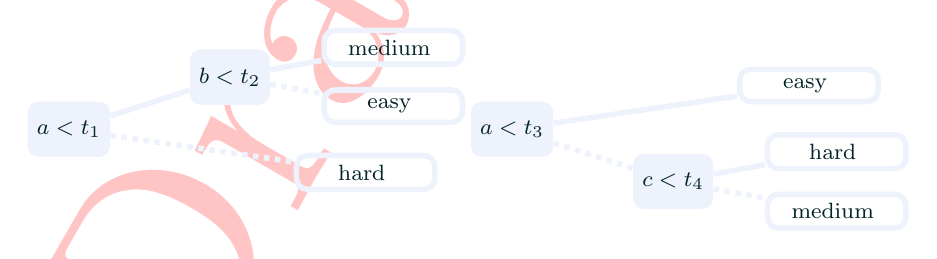
\begin{tikzpicture}[text=normalfg, 
	tree/.style = {fill=normalbg, rectangle, rounded corners, minimum width=2em, minimum height=2em}, 
    yes/.style = {draw=myblue, circle, align=center, inner sep=0em, minimum width=1em, text centered}, 
    no/.style = {draw=examplebg, circle, align=center, inner sep=0em, minimum width=1em, text centered}, 
    cl/.style = {draw=normalfg, circle, align=center, inner sep=0em, minimum width=1em, text centered}, 
    leaf/.style = {draw=normalbg, line width=2pt, rectangle, rounded corners, align=center, minimum width=5em, minimum height=1em, xshift=-1em},
    featl/.style = {draw=myblue, minimum width=1em, minimum height=1em},
    featr/.style = {draw=examplebg, minimum width=1em, minimum height=1em}]

% tree A
\node[tree] (Aa1) { \smaller $a < t_1$ };
\node[tree, above right=of Aa1, yshift=-3em] (Ab1) { \smaller $b < t_2$ };
\node[leaf, above right=of Ab1, yshift=-3.5em] (Ac1) { \smaller medium };
\node[leaf, below right=of Ab1, yshift=3.5em] (Ac2) { \smaller easy };
\node[leaf, below=1em of Ac2] (Ac3) { \smaller hard };

\node[right=of Ac1] {};

\draw[draw=normalbg, line width=2pt] (Aa1) -- (Ab1);
\draw[draw=normalbg, line width=2pt] (Ab1) -- (Ac1);
\draw[draw=normalbg, line width=2pt, dotted] (Aa1) -- (Ac3);
\draw[draw=normalbg, line width=2pt, dotted] (Ab1) -- (Ac2);

% tree B
\node[tree, right=13em of Aa1] (Ba1) { \smaller $a < t_3$ };
\node[tree, below right=of Ba1, yshift=3em] (Bb2) { \smaller $c < t_4$ };
\node[leaf, above right=of Bb2, yshift=-3.5em] (Bc3) { \smaller hard };
\node[leaf, below right=of Bb2, yshift=3.5em] (Bc4) { \smaller medium };
\node[leaf, above=1em of Bc3] (Bc2) { \smaller easy };

\draw[draw=normalbg, line width=2pt] (Ba1) -- (Bc2);
\draw[draw=normalbg, line width=2pt] (Bb2) -- (Bc3);
\draw[draw=normalbg, line width=2pt, dotted] (Ba1) -- (Bb2);
\draw[draw=normalbg, line width=2pt, dotted] (Bb2) -- (Bc4);


\end{tikzpicture}
\end{block}
\end{frame}


\begin{frame}{Encoding an Auxiliary SAT Instance}
Number of leaf combinations exponential in number of trees, but not all leaf combinations are \emph{possible}.
\begin{block}{Generate possible leaf combinations}
\begin{itemize}
\item Encoding all decision trees as described
\item For each feature $f$ add constraint: $\lnot fv_0 \lor \lnot fv_1 \lor \dots \lor \lnot fv_n$
\item Generate all solutions, projected to leaf variables
\end{itemize}

\medskip

\begin{center}
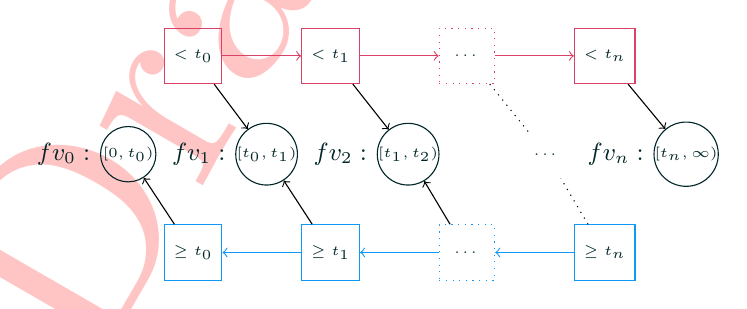
\begin{tikzpicture}[text=normalfg, 
	tree/.style = {fill=normalbg, rectangle, rounded corners, minimum width=2em, minimum height=2em}, 
    yes/.style = {draw=myblue, circle, align=center, inner sep=0em, minimum width=1em, text centered}, 
    no/.style = {draw=examplebg, circle, align=center, inner sep=0em, minimum width=1em, text centered}, 
    cl/.style = {draw=normalfg, circle, align=center, inner sep=0em, minimum width=1em, text centered}, 
    leaf/.style = {draw=normalbg, line width=2pt, rectangle, rounded corners, align=center, minimum width=5em, minimum height=1em},
    featl/.style = {draw=myblue, minimum width=2em, minimum height=2em},
    featr/.style = {draw=examplebg, minimum width=2em, minimum height=2em},
    inter/.style = {draw=normalfg, circle, align=center, inner sep=0em, minimum width=2em, minimum height=2em}]

\node (o) {};
\node[above=of o] (n) {};
\node[below=of o] (m) {};

\node[inter, right=of o, xshift=-2.3em] (f1i1) {\tiny $[0, t_0)$};
\node[inter, right=of f1i1] (f1i2) {\tiny $[t_0, t_1)$};
\node[inter, right=of f1i2] (f1i3) {\tiny $[t_1, t_2)$};
\node[inter, draw=none, right=of f1i3] (dots) {\tiny \dots};
\node[inter, right=of dots] (f1i5) {\tiny $[t_n, \infty)$};

\node[left=0em of f1i1] {\small $fv_0:$};
\node[left=0em of f1i2] {\small $fv_1:$};
\node[left=0em of f1i3] {\small $fv_2:$};
\node[left=0em of f1i5] {\small $fv_n:$};

\node[featl, right=of n] (f1l1) {\tiny $<t_0$};
\node[featl, right=of f1l1] (f1l2) {\tiny $<t_1$};
\node[featl, dotted, right=of f1l2] (f1l3) {\tiny \dots};
\node[featl, right=of f1l3] (f1l4) {\tiny $<t_n$};
\draw[->, draw=myblue] (f1l1) -- (f1l2);
\draw[->, draw=myblue] (f1l2) -- (f1l3);
\draw[->, draw=myblue] (f1l3) -- (f1l4);

\node[featr, right=of m] (f1r1) {\tiny $\geq t_0$};
\node[featr, right=of f1r1] (f1r2) {\tiny $\geq t_1$};
\node[featr, dotted, right=of f1r2] (f1r3) {\tiny \dots};
\node[featr, right=of f1r3] (f1r4) {\tiny $\geq t_n$};
\draw[<-, draw=examplebg] (f1r1) -- (f1r2);
\draw[<-, draw=examplebg] (f1r2) -- (f1r3);
\draw[<-, draw=examplebg] (f1r3) -- (f1r4);

\draw[->] (f1r1) -- (f1i1);
\draw[->] (f1r2) -- (f1i2);
\draw[->] (f1r3) -- (f1i3);
\draw[dotted] (f1r4) -- (dots);

\draw[->] (f1l1) -- (f1i2);
\draw[->] (f1l2) -- (f1i3);
\draw[dotted] (f1l3) -- (dots);
\draw[->] (f1l4) -- (f1i5);

\end{tikzpicture}
\end{center}
\end{block}
\end{frame}


\begin{frame}{Final Encoding of Random Forest Classifiers}

\begin{itemize}
\item Encoding all decision trees as described
\item Determine class $\kappa(M) \in K$ for each model $M$ of the auxiliary SAT instance (each solution is a \emph{possible} leaf combination)
\item $S_k := \{M \mid \kappa(M) = k \}$
\end{itemize}

\begin{block}{Monolithic Approach}

For each class $k \in K$, encode $k \rightarrow \bigvee\limits_{M \in S_k} \bigwedge\limits_{m \in M}m$

\end{block}


\begin{block}{Incremental Approach}

Incrementally build formula equisatisfiable to $k \rightarrow \bigvee\limits_{M \in S_k} \bigwedge\limits_{m \in M}m$

\begin{itemize}
\item add models in $S_k$ one by one and solve
\item needs additional encoding variables and use of an assumption literal
\end{itemize}

\end{block}

\end{frame}


\begin{frame}{Determine all Prime Implicants of Classifier}

Given a formula $F$, a model $P \models F$ is a prime implicant of $F$ iff it is subset minimal, i.e., $\nexists P' \subset P, P' \models F$. 


\begin{block}{Prime Implicants of our Random Forest Encoding}
\begin{itemize}
\item Minimal number of excluded value intervals for selected class(es)
\item NOT minimal number of case-distinctions for selected class(es)
\item Largest connected feature subspaces for selected class(es)
\end{itemize}
\end{block}

\end{frame}


\begin{frame}{Results: Decision Tree (SC 2020 Data)}

Predict fastest solver in \{kissat-unsat, relaxed-newtech\} from 56 features, Accuracy: ~79\%

\begin{block}{Numbers of Case Distinctions: Leaf Depths vs. Prime Implicants}
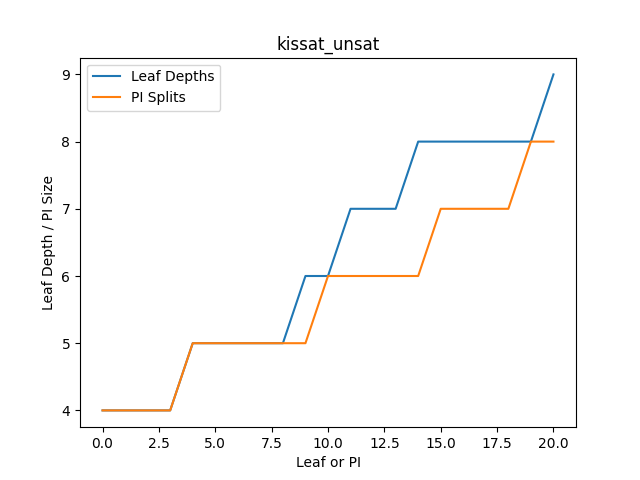
\includegraphics[width=.49\linewidth]{img/DT_kissatunsat_depth_vs_size.png}%
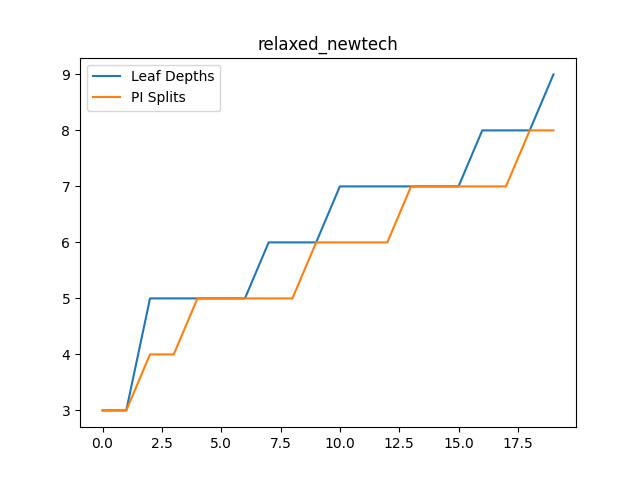
\includegraphics[width=.49\linewidth]{img/DT_relaxednewtech_depth_vs_size.png}
\end{block}

\end{frame}


\begin{frame}{Results: Random Forest, 2 Trees (SC 2020 Data)}
Predict fastest solver in \{kissat-unsat, relaxed-newtech\} from 56 features, Accuracy: ~74\%

\begin{block}{Prime Implicant: Numbers of Samples (left) Sizes (right)}
\begin{center}
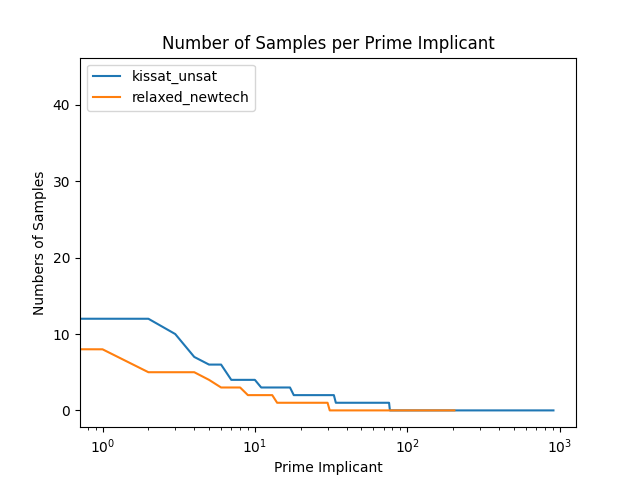
\includegraphics[width=.49\linewidth]{img/RF2_solvers_n_samples.png}%
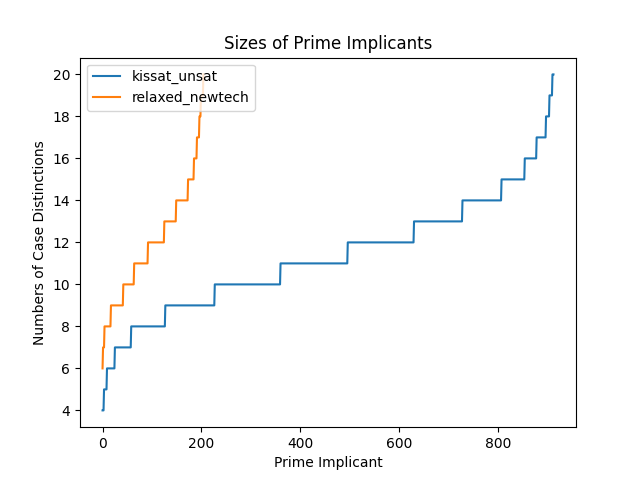
\includegraphics[width=.49\linewidth]{img/RF2_solvers_pi_sizes.png}
\end{center}
\end{block}

\begin{tabular}{ccc}
	\bf Leaf Comb. & \bf Possible Comb. & \bf PI computation\\
	\hline
	1554 & 1118 & 2 seconds\\
\end{tabular}
\end{frame}


\begin{frame}{Results: Random Forest, 3 Trees (SC 2020 Data)}
Accuracy: ~79\%

\begin{block}{Numbers of Samples}
\begin{center}
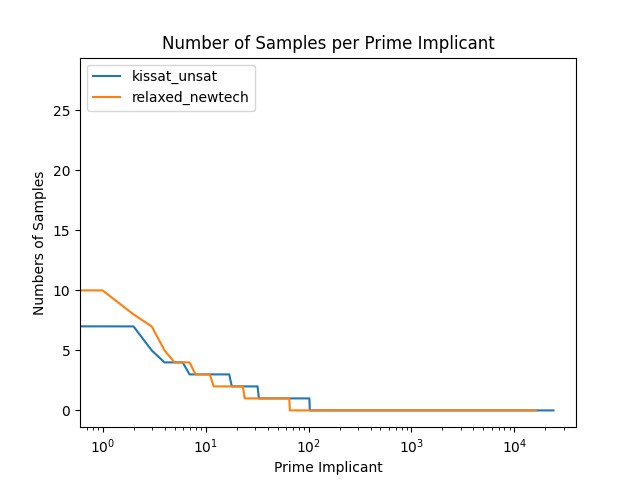
\includegraphics[width=.47\linewidth]{img/RF3_solvers_n_samples.png}%
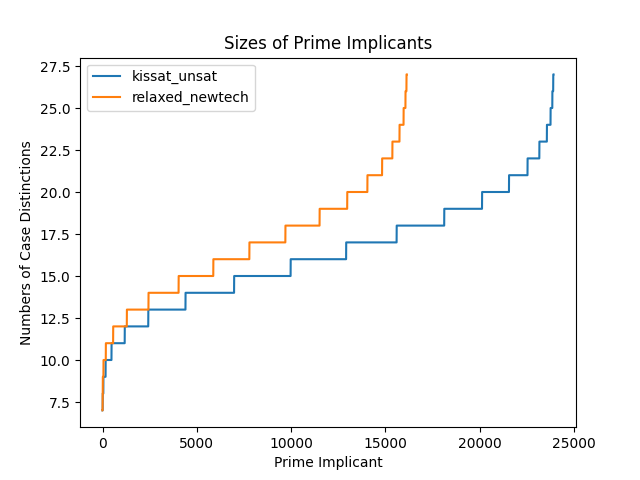
\includegraphics[width=.47\linewidth]{img/RF3_solvers_pi_sizes.png}
\end{center}
\end{block}

\begin{tabular}{ccrl}
	\bf Leaf Comb. & \bf Possible Comb. & \bf PI computation & code version\\
	\hline
	77700 & 40047 & 9518 seconds & original\\
	~ & ~ & ~50 seconds & C++\\
	~ & ~ & ~5 seconds & incremental
\end{tabular}
\end{frame}


\begin{frame}{Future Work}

\begin{block}{Parallelize and Approximate}
\begin{itemize}
\item Parallel and incremental enumeration of possible leaf combinations
\item Determine leaf combinations which are backed by samples
\item Analyze evolution of prime implicants while adding leaf combinations
\item Analyze evolution of accuracy through generalization
\end{itemize}
\end{block}

\begin{block}{Empirical Classes of SAT Instances}
\begin{itemize}
\item Analyze prediction models for algorithm portfolios
\item Feedback for algorithm engineers
\item Recurrent ISAC-like approach without unsupervised learning
\end{itemize}
\end{block}

\end{frame}


\end{document}




